
\chapter{Úvod do problematiky}

\section{RNA}

RNA (Ribonukleová kyselina) je typ nukleové kyseliny, která je nezbytná pro
různé biologické procesy. Skládá se z dlouhého řetězce nukleotidů obsahujících
cukr, fosfátovou skupinu a dusíkatou bázi. Čtyři dusíkaté báze v RNA jsou
adenin, guanin, cytosin a uracil. RNA je transkribována z DNA a může být
nalezena všude v živých buňkách.

\subsection{Funkce}

RNA má několik důležitých funkcí v buňkách. Jednou z jejích hlavních funkcí je
fungovat jako posel mezi DNA a ribozomy během syntézy proteinů. Messenger RNA
(mRNA) nese genetickou informaci z DNA k ribozomům, které tuto informaci
používají k vytváření proteinů. Další typy RNA, jako tRNA a rRNA, hrají také
důležité role v syntéze proteinů.

Nekódující RNA (ncRNA) je druh RNA, která nekóduje proteiny, ale místo toho
hraje regulační role v buňkách. ncRNA lze rozdělit do dvou širokých kategorií:
malé ncRNA, které jsou menší než 200 nukleotidů, a dlouhé ncRNA, které jsou
delší než 200 nukleotidů. Malé ncRNA, jako jsou mikroRNA a siRNA, se účastní
po-transkripční regulace genů, zatímco dlouhé ncRNA se účastní různých
buněčných procesů, včetně regulace exprese genů, remodelace chromatinu a
inaktivace chromozomu X. Dysregulace ncRNA byla spojena s několika nemocemi,
včetně rakoviny a neurodegenerativních onemocnění.

\subsection{Sekundární struktura RNA}

Sekundární struktura RNA se týká způsobu, jakým se molekula RNA skládá díky
párovacím interakcím mezi komplementárními nukleotidy. Existuje několik běžných
typů (motivů) sekundárních struktur, které může RNA tvořit.

\subsubsection{Motivy sekundární struktury RNA}

\paragraph{Hairpin loop}

Jedním z nejčastějších typů sekundární struktury je hairpin loop, který se
skládá z jednořetězcové oblasti RNA, která se ohýbá zpět na sebe a vytváří kmen
(dvouřetězcovou oblast) a smyčku (jednořetězcovou oblast). Hairpin smyčky se
často nacházejí na koncích molekul RNA a mohou hrát důležité role v stabilitě a
zpracování RNA.

\begin{figure}[H]
  \centering
  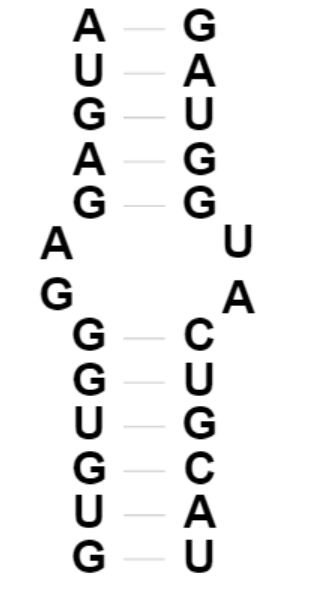
\includegraphics[height=40mm]{../img/kap01/rna/hairpin.png}
  \caption{Ukázka motivu hairpin loop}
\end{figure}

\paragraph{Bulge}

Dalším častým typem sekundární struktury je bulge, který zahrnuje jeden
nukleotid, který není spárovaný s komplementárním nukleotidem v kmenové
oblasti. Bulges mohou narušit sekundární strukturu RNA, ale také mohou být
důležité v interakci mezi proteinem a RNA.

\begin{figure}[H]
  \centering
  
\includegraphics[width=20mm]{../img/kap01/rna/bulge.png}
  \caption{Ukázka motivu bulge}
\end{figure}

\paragraph{Multibranch loop}

Multibranch loop je složitější sekundární struktura, která zahrnuje tvorbu více
stonků a smyček. Tyto struktury mohou být důležité pro skládání a funkci RNA a
často se nacházejí v molekulách RNA s katalytickou aktivitou, jako jsou
ribozymy.

\begin{figure}[H]
  \centering
  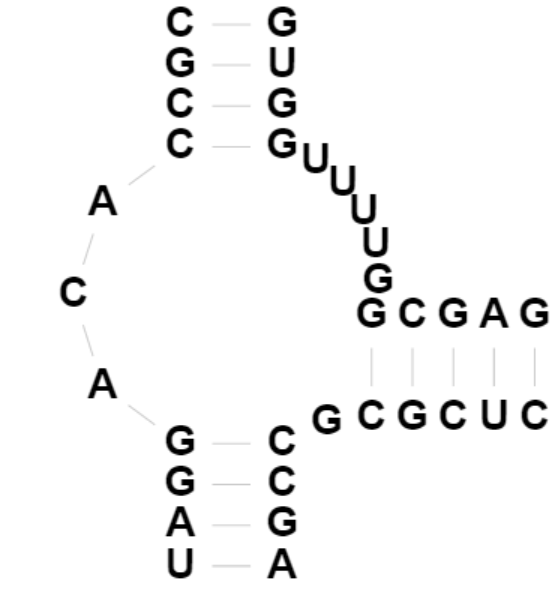
\includegraphics[height=40mm]{../img/kap01/rna/multibranch.png}
  \caption{Ukázka motivu multibranch loop}
\end{figure}

Celkově je pochopení sekundární struktury RNA zásadní pro pochopení její
biologické funkce a toho, jak interaguje s jinými molekulami v buňce.

\section{Vizualizace sekundárních RNA struktur} 

Pro reprezentaci sekundární RNA struktury se používají jak textové, tak
grafické způsoby, ale ty grafické slouží mnohem lépe k analýze struktur.
Třídimenzionální reprezentace sekundárních RNA struktur je sice nejpřesnější,
ale je složité jí získat a proto se stále nejvíce používají dvoudimenzionální
reprezentace. 

V této části představíme tři nejpoužívanější reprezentace - arc diagram,
circular diagram a radiate diagram. Obrázky ukázek diagramu v této části jsou
získané za pomoci nástroje VARNA\cite{Varna}.

V arc diagramu jsou nukleotidy zobrazeny na rovné čáře ve stejném pořadí jako v
sekvenci a bázové páry nukleotidů jsou spojeny obloukem.

\begin{figure}[H]
  \centering
  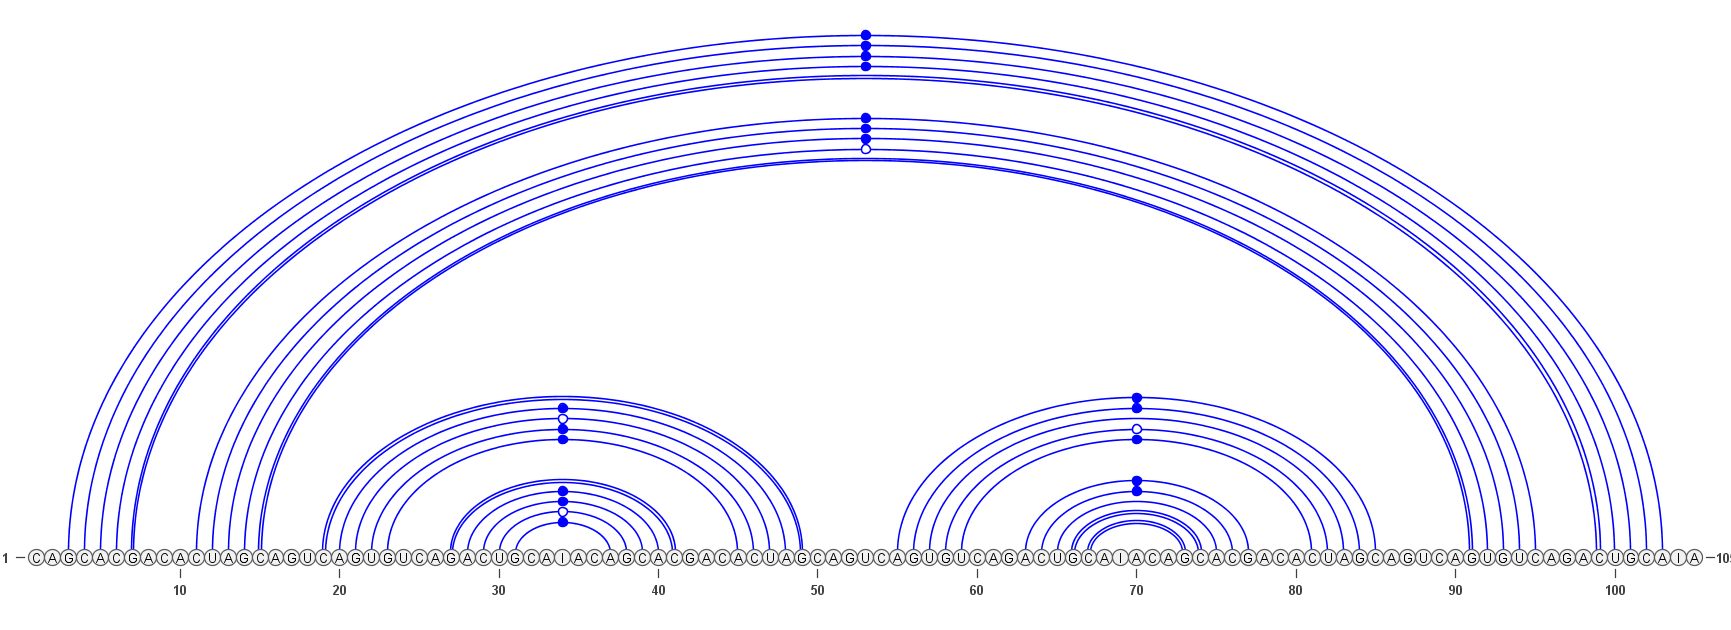
\includegraphics[width=140mm]{../img/kap01/diagrams/arc.png}
  \caption{Ukázka arc diagramu}
\end{figure}

Circular diagram je velmi podobný. Nukleotidy neleží na rovné čáře, ale po
obvodu kruhu. Bázové páry jsou spojeny buď čárou nebo obloukem.

\begin{figure}[H]
  \centering
  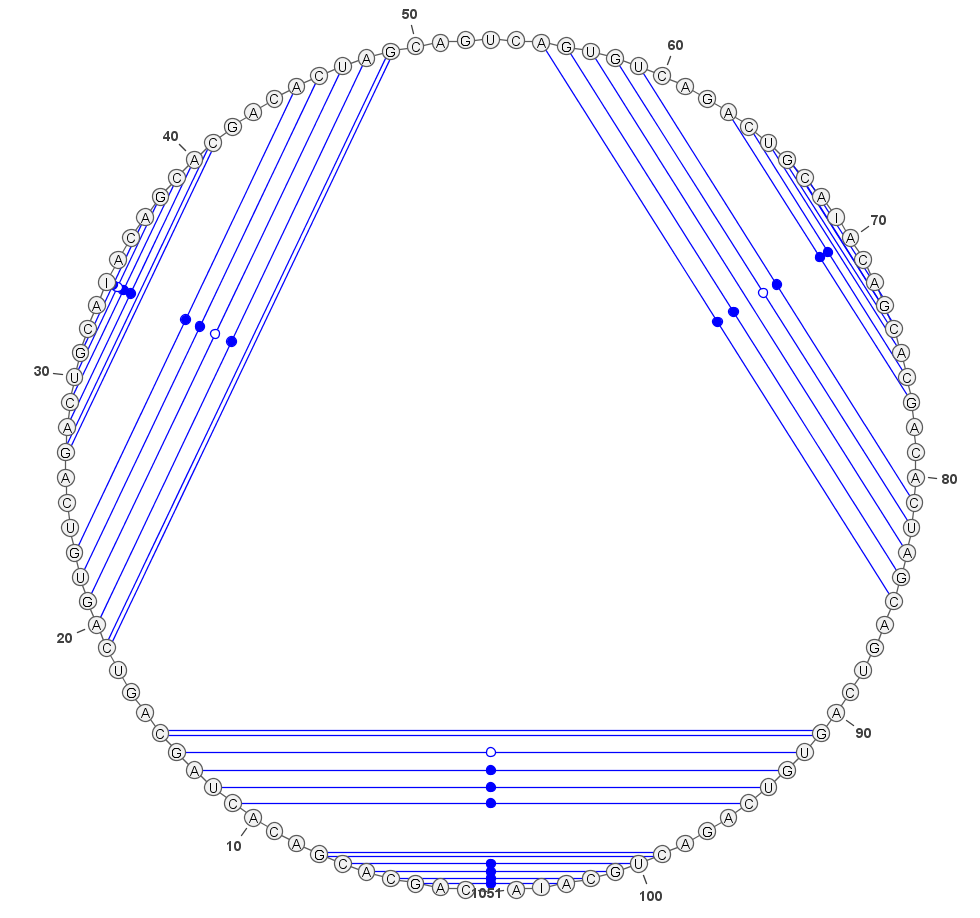
\includegraphics[height=100mm]{../img/kap01/diagrams/circular.png}
  \caption{Ukázka circular diagramu}
\end{figure}

V radiate diagramu jsou pozice nukleotidů voleny tak, aby bylo možné rozeznat
motivy sekundární struktury, jako jsou hairpins, bulges nebo multibranch loops. 

\begin{figure}[H]
  \centering
  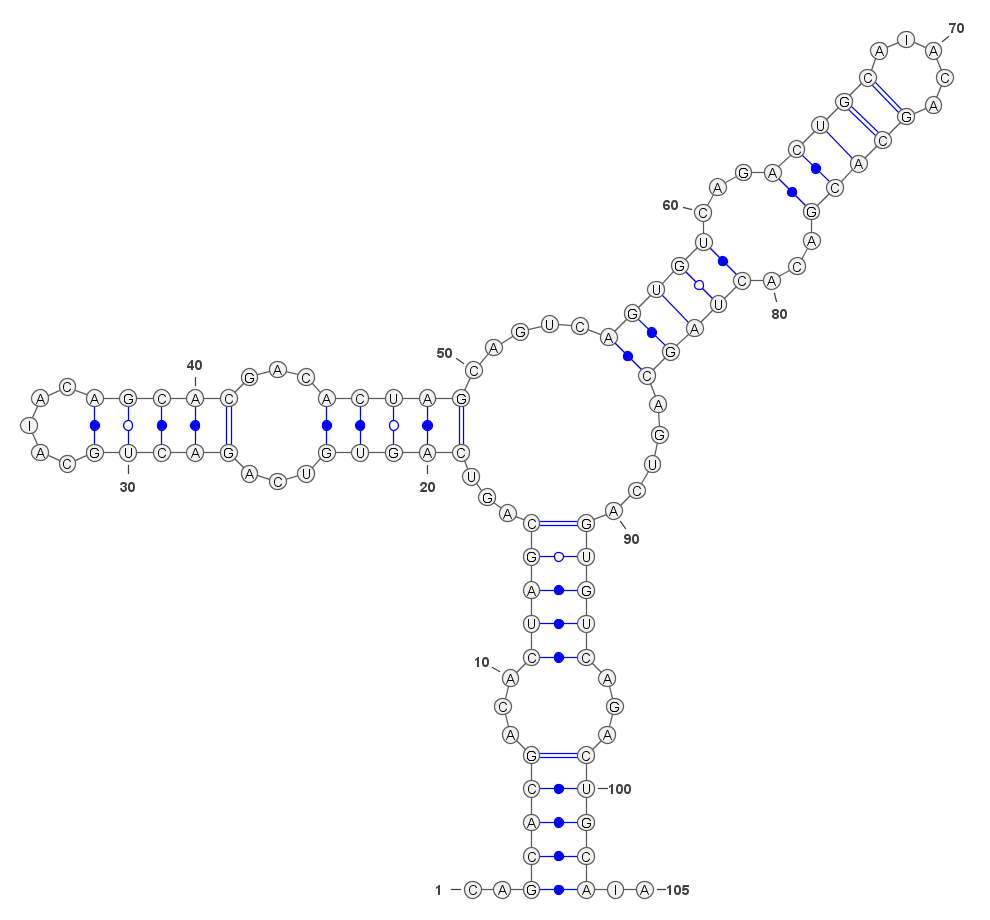
\includegraphics[height=100mm]{../img/kap01/diagrams/radiate.png}
  \caption{Ukázka radiate diagramu}
\end{figure}

Právě schopnost zachytit zmíněné motivy obě předešlé reprezentace postrádají, a
proto se radiate diagram používá tam, kde je potřeba detailní vizuální analýza
motivů sekundární RNA struktury a její interakce. 


\section{Podobné projekty} {\color{red} chybi motivacni uvod, ktery by rekl, co chceme delat, aby bylo mozne pochopit podobne k cemu}

Rádi bychom čtenáře seznámili s některými nástroji, které jsou používané pro
vizualizaci sekundárních RNA struktur. Většina z nich jsou programy s
uživatelským rozhraním a mohlo by se proto zdát zbytečné je zmiňovat nebo
porovnávat s naší knihovnou. Nicméně u níže zmíněných programů není důležité
řešení samotného uživatelského rozhraní, jako především druh zvolených metod
pro vizualizaci a následné porovnávání.

Z velkého množství existujících nástrojů, byla snaha vybrat takové,
které mají rozdílné přístupy a nabízí nejširší paletu funkcí.

\subsection{VARNA} 

VARNA (Visualization Applet for RNA) je nástroj pro automatické
kreslení, vizualizaci a anotaci sekundárních RNA struktur, navržený jako
doprovodný software pro webové servery a databáze.

VARNA implementuje algoritmy pro vykreslení všech tří výše zmíněných diagramů,
podporuje různé textové formáty pro vstup i výstup a je schopný exportovat
kresbu do rastrových nebo vektorových formátů. Umožňuje ruční úpravy a
strukturální anotace výsledku kresby a je považován za standard pro práci se
sekundárními strukturami RNA.

\begin{figure}[H]
  \centering
  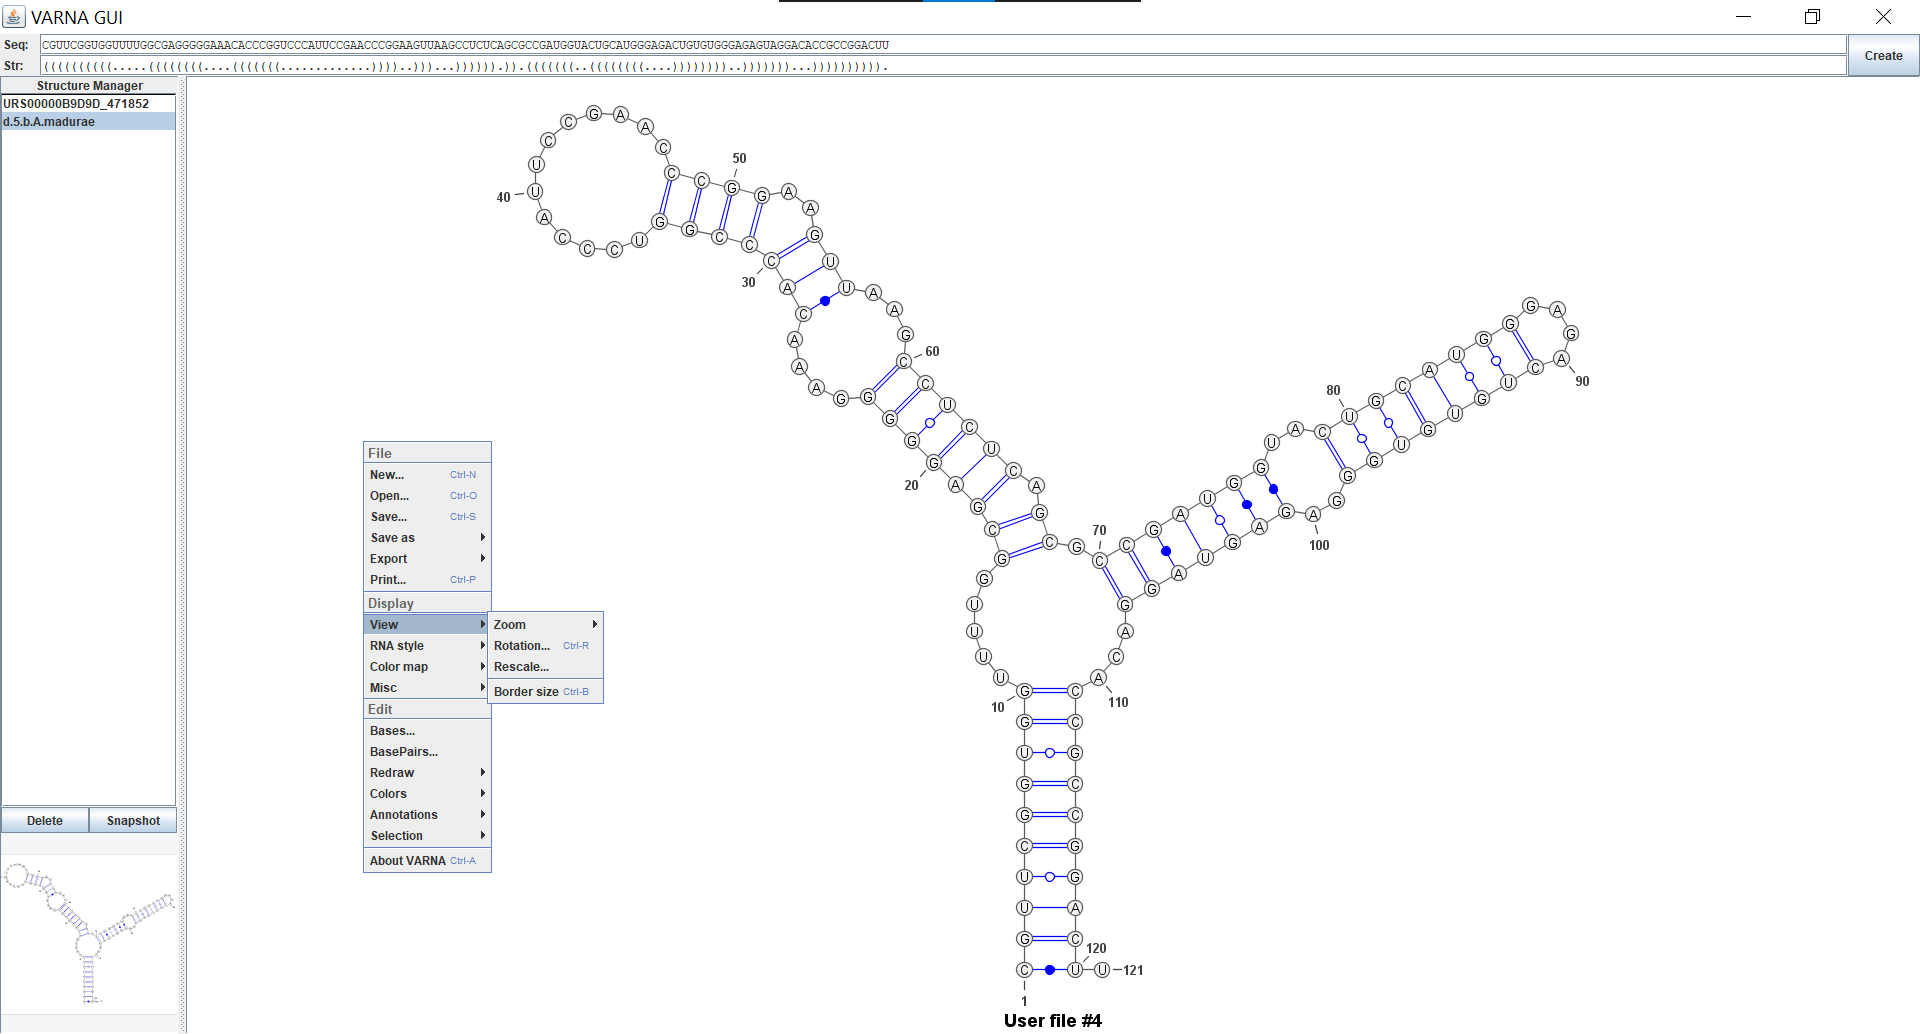
\includegraphics[width=140mm]{../img/kap01/tools/varna.png}
  \caption{Snimek nástroje Varna. Zobrazená struktura je d.5.b.A.madurae.}
\end{figure}

\subsection{RNAStructViz} 

RNAStructViz\cite{RnaStructViz} je grafický nástroj pro analýzu sekundárních
RNA struktur. Jeho předností je vizuální porovnání tří konfigurací v circular
arc diagramu. Doplněné zabudovaným prohlížečem CT-style\footnote{CT formát
souboru slouží k ukládání informace o sekvenci a bázových párů.} souboru a
prohlížečem radial diagramu podstruktury, která je přímo propojená s arc
diagram oknem skrze nástroj pro výběr zoom. Mezi další funkce patří vypočítání
číselných informací a možnost exportu obrázků a dat pro pozdější použití.

\begin{figure}[H]
  \centering
  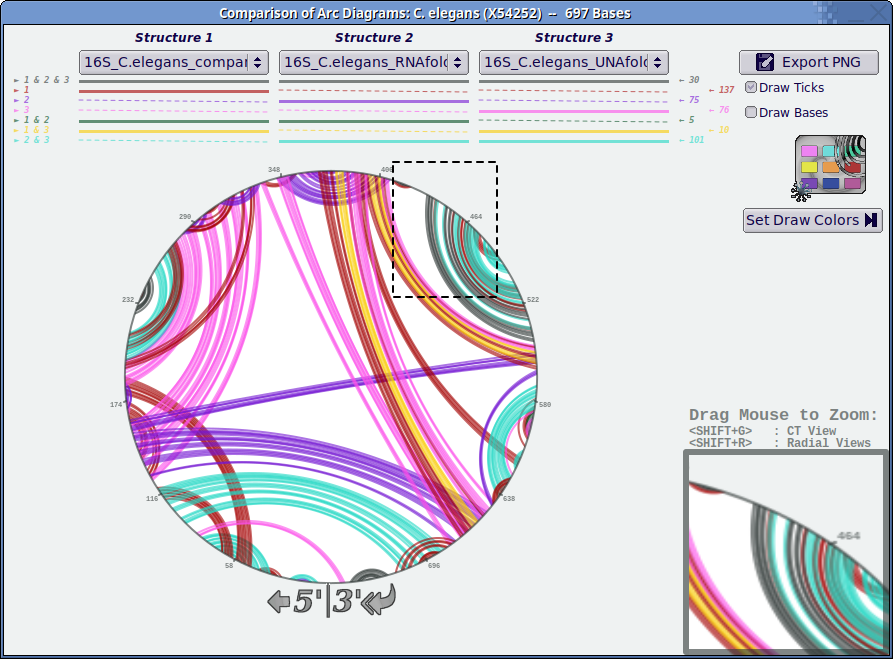
\includegraphics[width=140mm]{../img/kap01/tools/rnaStructViz.png}
  \caption{Snimek nástroje rnaStructViz, zobrazující tři struktury RNA.}
\end{figure}

\subsection{Forna} 

Forna\cite{Forna} (force-directed rna) nabízí webové rozhraní a server, který
umožňuje uživateli vložit sekundární RNA strukturu ve formátu dot-bracket a
zobrazí ji jako force-directed
graf\footnote{https://cs.brown.edu/people/rtamassi/gdhandbook/chapters/force-directed.pdf}.
Uživatel může následně upravit pozice přetažením myší a lze i upravovat přímo
strukturu. 

\begin{figure}[H]
  \centering
  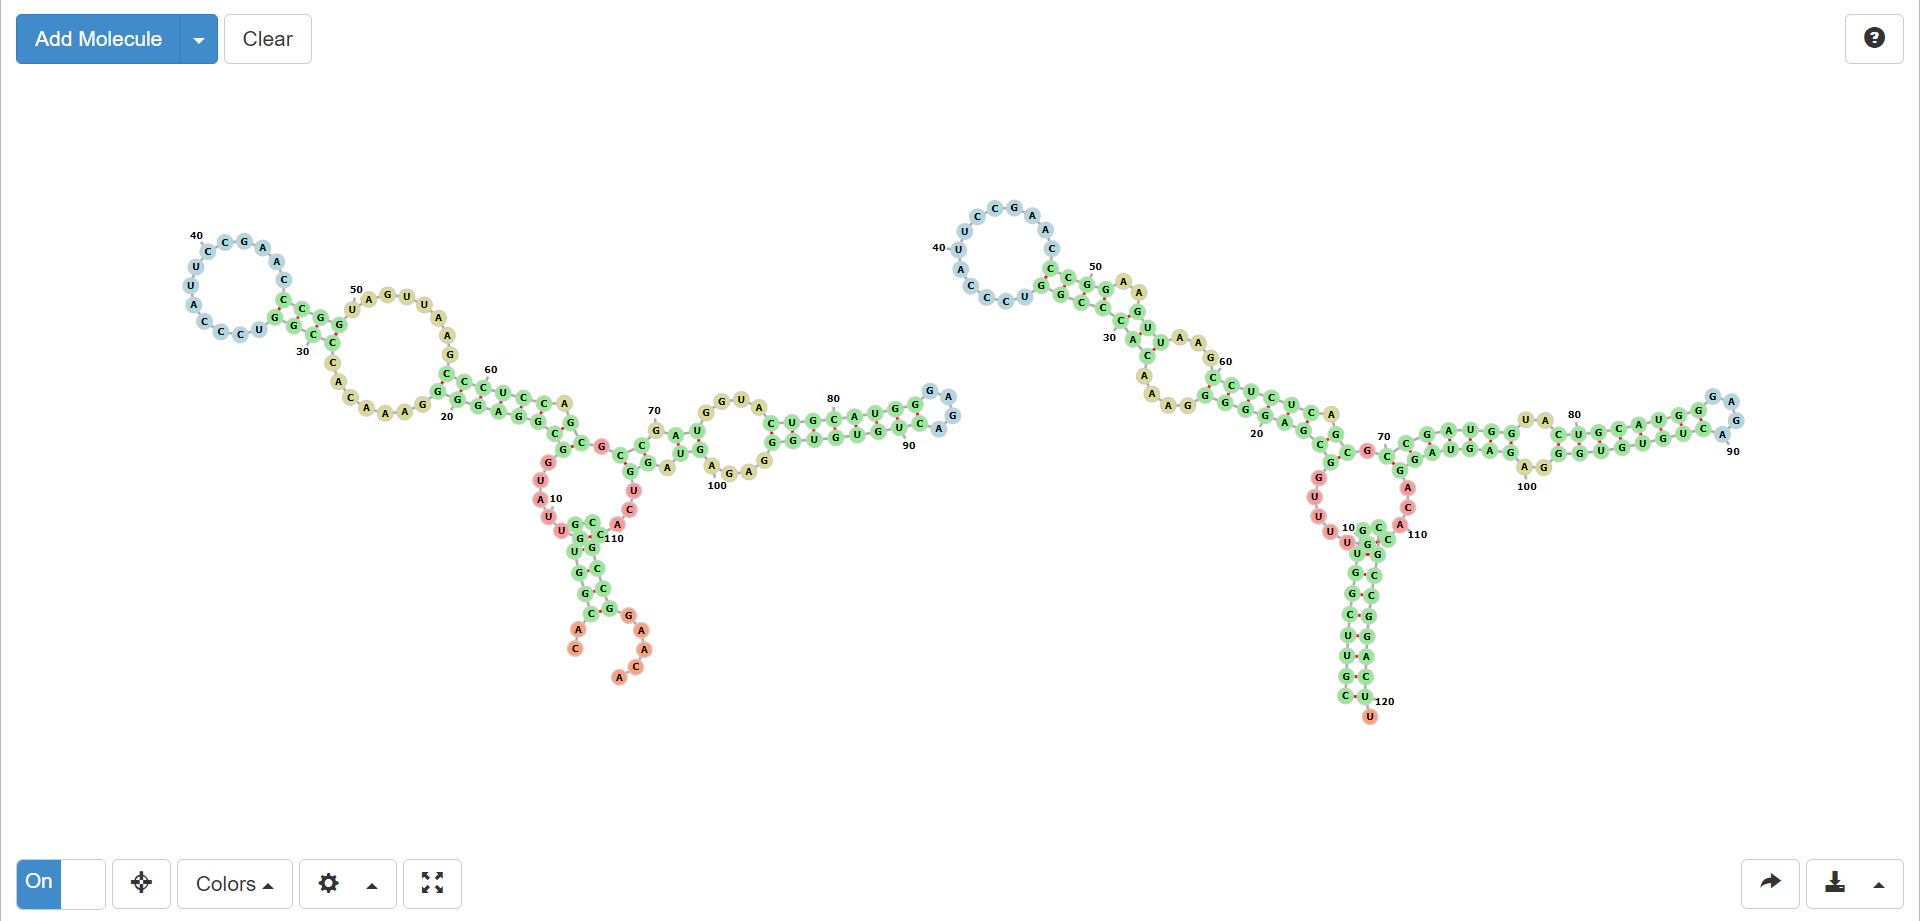
\includegraphics[width=140mm]{../img/kap01/tools/forna.png}
  \caption{Snimek nástroje Forna. Nalevo odvozená sekundární RNA
  struktura URS00000B9D9D\_471852 od struktury d.5.b.A.madurae napravo.}
\end{figure}

\subsection{R-chie} 

R-chie \cite{Rchie} je web server, který umí vygenerovat šest různých typů arc
diagramu. Vývoj tohoto nástroje byl se zaměřením především na složitější
struktury, které nelze hezky nakreslit v radial diagramu. R-chie umí
vygenerovat diagram pro porovnávání dvou sekundárních RNA struktur. Důležitým
cílem byla možnost generovat diagramy pro velké množství dat, proto také
nenabízí grafické rozhraní a s ním spojenou interakci se strukturami. 

Projekt také nabízí balíček napsaný v jazyce
R\footnote{https://www.r-project.org/} zvaný R4RNA, který umožňuje spuštění
programu lokálně a napříč operačním systémům.

\begin{figure}[H]
  \centering
  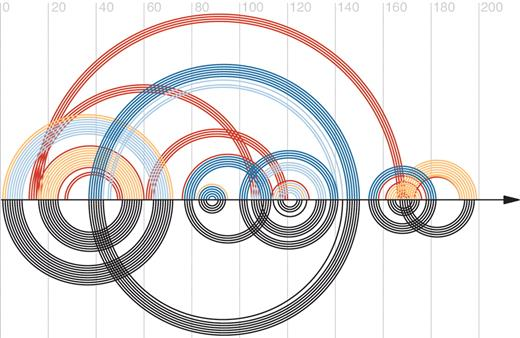
\includegraphics[width=140mm]{../img/kap01/tools/rchie.jpeg}
  \caption{Výsledný arc diagram nástroje R-chie, zobrazující dvě sturktury.
  První struktura je nad horizontální čárou a druhá pod ní.}
\end{figure}

\subsection{Shrnutí existujících nástrojů}

Nástroje představené v této kapitole se soustředí především na práci s circular
diagramem nebo arc diagramem, a právě pouze pro tyto diagramy nabízí nějaké
metody pro porovnávání omezeného množství sekundárních struktur RNA. Forna
podporuje pouze radial diagram, ale porovnávání dvou struktur, které sice jdou
zobrazit vedle sebe, už nijak neusnadňuje. 

Varna Podporuje všechny tři zmíněné diagramy, ale nelze ani zobrazit dvě
sekundární RNA struktury vedle sebe. Velkou výhodou nástroje VARNA by byla
možnost použití na webu, ale k tomu používá Java Applets
\footnote{https://docs.oracle.com/javase/tutorial/deployment/applet/index.html},
které jsou od roku 2017 považované za zastaralé
\footnote{https://www.oracle.com/java/technologies/javase/9-deprecated-features.html}.

Ze zmíněných projektů je nejpodobnější tomu našemu R-chie, který se snaží
usnadnit porovnávání sekundárních RNA struktur a nabízí i knihovnu napsanou v
jazyce R. Liší se pak v samotném přístupu, protože jejich rozhraní generuje
pouze statické circular nebo arc diagramy.

\section{Kreslení grafů na základě šablony}

Níže jsou zmíněné dva projekty, které úzce souvisí s naší knihovnou, protože
produkují data ve formátu, se kterým pracuje naše knihovna a metody
použité ke generovaní takových dat jsou klíčové pro naší knihovnu.

\subsection{TRAVeLer} 

Traveler\cite{Traveler2017} je nástroj pro vizualizaci cílové sekundární
struktury, využívající existující rozložení dostatečně podobné RNA struktury
jako vzor. Traveler je založený na algoritmu, který konvertuje cílovou a
vzorovou strukturu do odpovídající stromové reprezentace a využije stromovou
editační vzdálenost společně s modifikací rozložení k přetvoření vzorové
struktury do cílové. Traveler přijme na vstupu sekundární strukturu a vzor
rozložení a na výstupu dá rozložení cílové struktury. Je to tedy command-line
open source nástroj schopný rychle generovat rozložení i pro největší RNA
struktury za poskytnutí dostatečně podobného rozložení.

Do vzniku Traveleru neexistoval žádný nástroj, který by dokázal velké struktury
vizualizovat ve standardní notaci, se kterou jsou biologové naučení pracovat a
porovnávat struktury napříč druhům.

\begin{figure}[H]
  \centering
  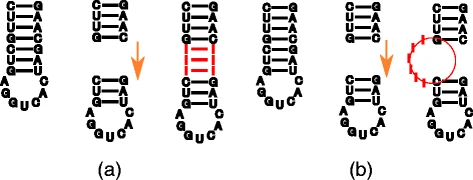
\includegraphics[width=100mm]{../img/kap01/editation.png}
  \caption{Ilustrace jednoduchých editací vzorové struktury.}
\end{figure}

\subsection{R2DT} 

R2DT\cite{R2DT2021} je metoda pro predikci a vizualizaci široké škály
sekundárních RNA struktur ve radial diagramu. R2DT je postaveno na knihovně se
3 647 vzory reprezentujícími většinu známých RNA struktur. R2DT se používá na
ncRNA sekvencích z RNAcentral\footnote{https://rnacentral.org/} databáze a
vytvořila více než 27 miliónů diagramů\footnote{Číslo je aktuální k datu 11.4.
2023}, čímž tvoří největší světovou sadu dat s 2D RNA strukturami. Pro
vizualizaci neboli 2D rozložení používá R2DT právě výše zmíněný nástroj
Traveler.
